%results & evaluation, explicitly mentioning of known limitations

So far, we are able to fully generate terrains, including elevations, biomes and rivers.
Figure~\ref{fig:generator} shows a generated map.

\begin{figure}[H]
	\centering
	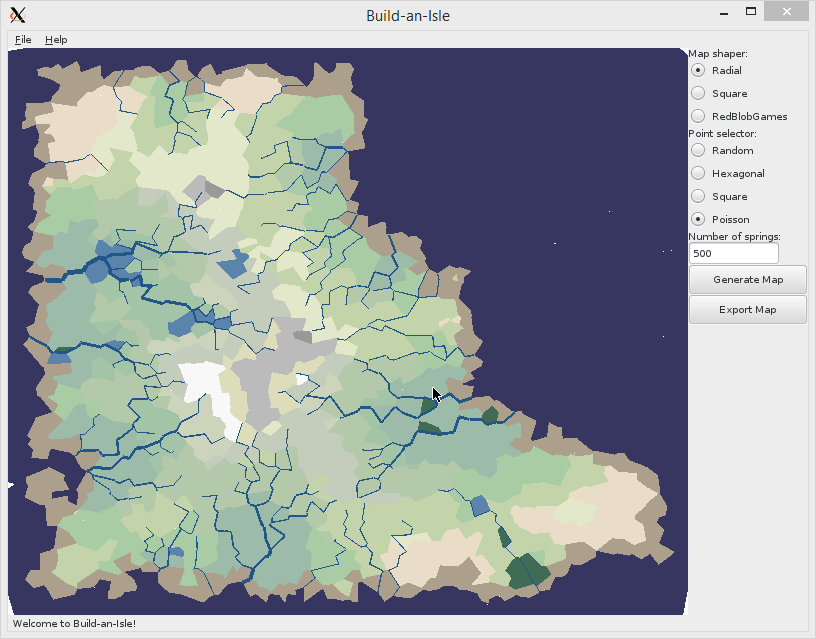
\includegraphics[width=0.8\linewidth]{topdown}
	\caption{A generated map}
	\label{fig:generator}
\end{figure}

\begin{figure}[H]
	\centering
	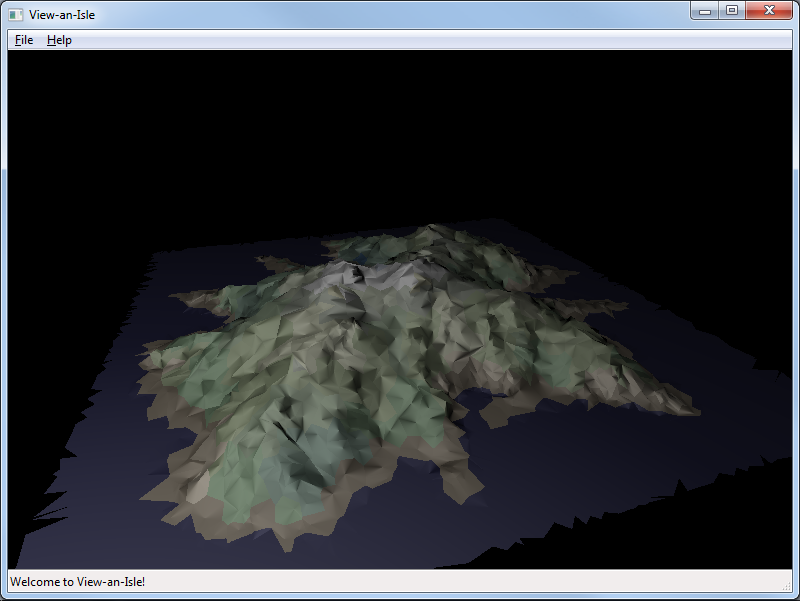
\includegraphics[width=0.8\linewidth]{resultsmallnorivers}
	\caption{A small map without rivers for which geometry has been generated}
	\label{fig:generator}
\end{figure}

\begin{figure}[H]
	\centering
	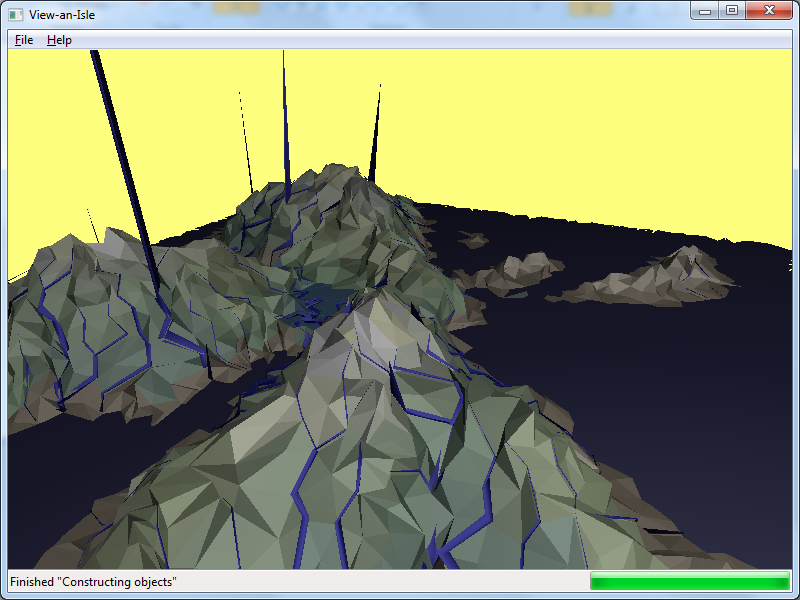
\includegraphics[width=0.8\linewidth]{shamefulldisplay}
	\caption{There are cases where rivers can be visualised without standing out, however many of the generated maps will contain small polygons that lead to unpredictable geometric river representations. It would take a significant amount of time to improve the current method.}
	\label{fig:generator}
\end{figure}

\begin{figure}[H]
	\centering
	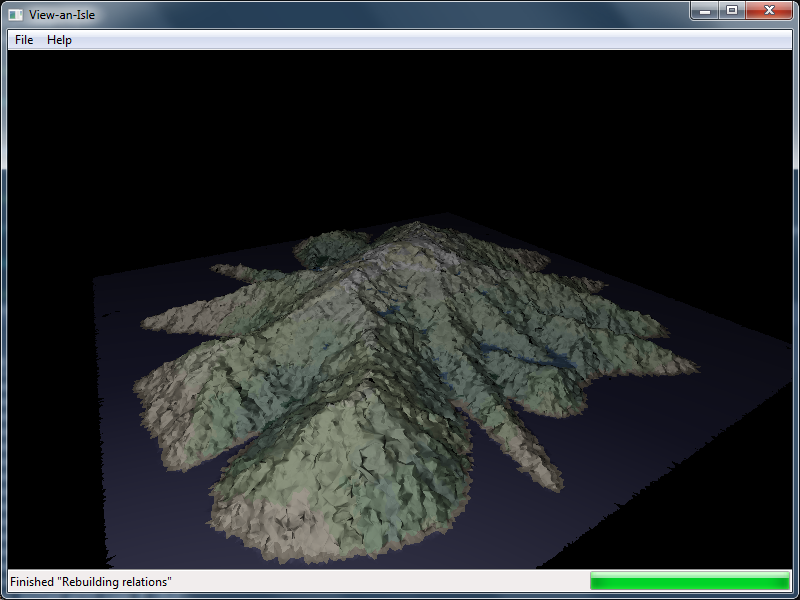
\includegraphics[width=0.8\linewidth]{resultlargenorivers}
	\caption{A large map showcasing a body of water situated high above sea level}
	\label{fig:generator}
\end{figure}

We have also started work on the viewer, although that is not yet as interactive as it should be.
